\documentclass[a4paper]{article}
\usepackage[T1]{fontenc}
\usepackage[utf8]{inputenc}
\usepackage[italian]{babel}
\usepackage{float}
\usepackage{subcaption}
\usepackage{enumitem}
\usepackage{graphicx}
\usepackage{makecell}
\graphicspath{{./images/}}
\usepackage{tabularx}
%\usepackage{geometry} 
%\geometry{a4paper,top=3cm,bottom=3cm,left=3.5cm,right=3.5cm,% heightrounded,bindingoffset=5mm}

\begin{document}

\author{Manuel Trivilino, Davide Salaorni, Luca Terracciano}

\title{\Large \textbf{Data4Help RASD}\\
\textbf{Requirements Analysis and \\Specification Document}
    \begin{figure}[h]
        \centering
        
\includegraphics[width=270pt]{data4helpblu}
        \label{fig:my_label}
    \end{figure}
    \vspace{-2.4cm}
    \begin{figure}[h]
        \centering
        \includegraphics[width=200pt]{AutomatedSOSlogo.png}
        \label{fig:my_label}
    \end{figure}
    \vspace{-2cm}
    \begin{figure}[h]
        \centering
        \includegraphics[width=150pt]{Track4Runlogo}
        \label{fig:my_label}
\end{figure}
}

\maketitle
\newpage

\tableofcontents
\newpage

\section{Introduction}

\subsection{Purpose}
The purpose of this document is to describe the software-based solutions that TrackMe wants to offer to its customers. First of all, the system is analyzed in terms of description of the problem and analysis of goals, requirements and constraints. After that, a solution is modeled in terms of software and hardware constraints paying attention also to some implementation details. This document is addressed to the developers who will implement this solution.

\subsection{Scope}

\paragraph{Description of the given problem}

\paragraph{}
TrackMe is a company that develops software-based services for third parties and for consumers. The main service is called Data4Help.
 Data4Help is a service that allows third parties to monitor the location and the health status of individual, it handles a policy of permissions for each user and collects individual’s data from their personal devices.
The service supports the registration of individuals who, by registering, agree that TrackMe acquires their data. After registration, these third parties can request:

\begin{itemize}
    \item Access to the data of some specific individuals (we can assume, for instance, that they know an 
    individual by his/her social security number or fiscal code in Italy). In this case, TrackMe passes 
    the request to the specific individuals who can accept or refuse it.
    
    \item Access to anonymized data of groups of individuals (for instance, all those living in a certain 
    geographical area, all those of a specific age range, etc.). These requests are handled directly 
    by TrackMe that approves them if it is able to properly anonymize the requested data. For 
    instance, if the third party is asking for data about 10-year-old children living in a certain street 
    in Milano and the number of these children is two, then the third party could be able to derive 
    their identity simply having people monitoring the residents of the street between 8.00 and 
    9.00 when kids go to school. Then, to avoid this risk and the possibility of a misuse of data,
    TrackMe will not accept the request. For simplicity, we assume that TrackMe will accept any 
    request for which the number of individuals whose data satisfy the request is higher than 
    1000.

\end{itemize}

\paragraph{}
As soon as a request for data is approved, TrackMe makes the previously saved data available to the 
third party. Also, it allows the third party to subscribe to new data and to receive them as soon as 
they are produced.
TrackMe develops itself two third-party services: AutomatedSOS and Track4Run.

\paragraph{Goals}

\begin{enumerate}[label*={G.\arabic*}]
    
    %Data4Help
    
    \item Allow customers' registration.
    \begin{enumerate}[label*=.\arabic*]
        \item Registration can be done as individual user.
        \item Registration can be done as third party.
    \end{enumerate}
    
    \item Third parties can request for anonymized data.

    \item Third parties can subscribe to the service in order to periodically receive new data.
        
    \item Third parties can receive for a individual user's data.
    
    %AutomatedSOS
    \item Users' health status is continuously checked in AutomatedSOS and in case of it overcomes a certain threshold values an ambulance is called within 5 seconds.
    
    %Track4Run
    \item Users can organize a run.
    \item Users can enroll to a run.
    \item Users can be spectators of a run seeing the partecipants' position on a map.
    
\end{enumerate}

\clearpage

\subsection{Definitions, Acronyms, Abbreviation}

\subsubsection{Definitions}
    
    \begin{itemize}
        \item \textit{Customer:} generic person not registered in any of the services provided by TrackMe. 
        \item \textit{User:} person registered in at least one of the services provided by TrackMe.
        \item \textit{Third Party:} person or company registered in Data4Help that want to access to access to the service in order to acquire data.
        \item \textit{Individual Data:} data that belongs to a specific user: personal information and data acquired from their devices (i.e. location, health status, etc.).
        \item \textit{Anonymazed Data} aggregated data acquired from a group of users with specific characteristics without keeping track of who they belong to.
        \item \textit{Ambulance Dispatcher:} the contact center that handles the health care service and the ambulance allocation.
        \item \textit{Google Maps:} web mapping service developed by Google, it offers satellite imagery, street maps etc.
        \item \textit{Push Notification Service:} web service that offers a fast and secure channel to notify and exchange messages on the web.
    \end{itemize}
    
    \subsubsection{Acronyms}
    
    \begin{itemize}
        \item \textit{RASD:} Requirement, Analysis and Specification Document
        \item \textit{GPS:} Global Position System
        \item \textit{API:} Application Programming Interface
    \end{itemize}
    
    \subsubsection{Abbreviation}
        \begin{itemize}
        \item \textit{G.n} Goal number n
        \item \textit{D.n} Domain assumption number n
        \item \textit{R.n} Requirement number n
    \end{itemize}

\subsection{Document Structure}
The RASD is composed by:
\begin{enumerate}
    \item Explanation of the given problem, the analysis in terms of goals and it gives some information in order to better understand all the other document's parts.
    \item Describes the solution structure identifying it's general organization, the users, the operating environment and the major design and implementation constraints.
    \item The software implementation is analyzed paying attention to the software and hardware details adding also a description in terms of functional requirements, scenarios and use cases.
    \item The system is analyzed both in its static aspects and the dynamic ones using a specific formal modeling language, Alloy, in which the most important features are analyzed in order to verify if every constraint of the system is not violated.
\end{enumerate}

\section{Overall Description}

\subsection{Product Perspective}

\begin{figure}[H]
    \centering
    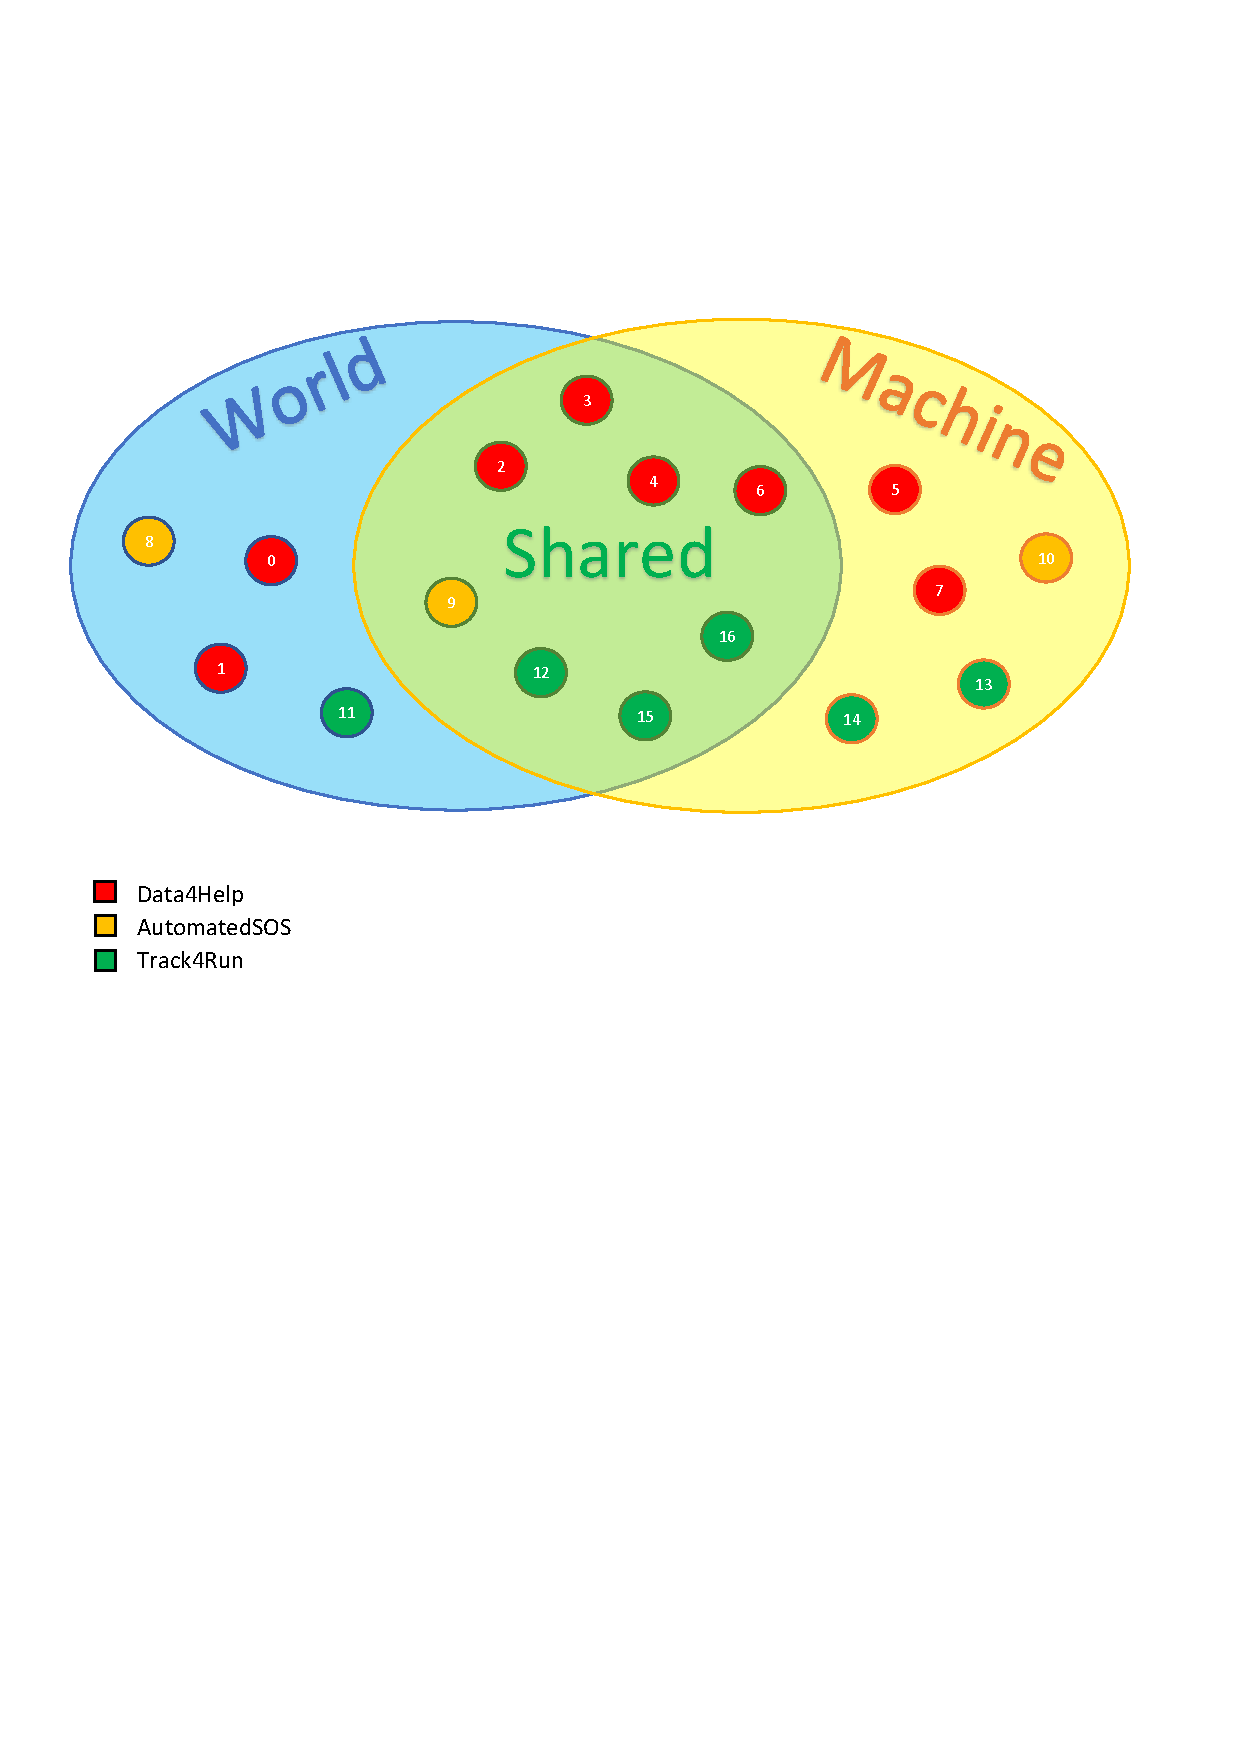
\includegraphics[width=\linewidth]{worldMachineShared-small}
    \caption{World, machine and shared phenomena.}
    \label{fig:my_label}
\end{figure}

\begin{enumerate} \itemsep=2pt
    \item [0.] User's location.
    \item [1.] User's health.
    \item [2.] Collecting data from smart devices.
    \item [3.] User's registration (agreement to share anonymized data).
    \item [4.] Data request from Third Party.
    \item [5.] Checking the anonymized data threshold.
    \item [6.] User's agreement for individual data share.
    \item [7.] Keeping track of connection between user and Third Party.
    \item [8.] Ambulance.
    \item [9.] Ambulance notification.
    \item [10.] Health status monitoring.
    \item [11.] Run event.
    \item [12.] Run creation and path definition.
    \item [13.] Run management and organization.
    \item [14.] Runner's registered position.
    \item [15.] View of the run event.
    \item [16.] Enrollment to the run.
\end{enumerate}

\clearpage


\subsection{Product Functions}
The main function that the system must perform are divided in three section, one for each software components.
\begin{itemize}
    \item Data4Help
    \begin{enumerate}
        \item Allow users to share their personal data with Data4Help and with the third parties who require them.
        \item Allow third parties to require users' data in anonymous form by using filters and offers the possibility to make a subscription to the request.
        \item Third parties can request for a specific user's data.
        \item Users can decide whether accept or not a data request from a third party.
    \end{enumerate}
    \item AutomatedSOS
    \begin{enumerate}
        \item Offers to the registered users to have their health status be continuously monitored.
        \item If the system detects an emergency situation it notifies an ambulance.
    \end{enumerate}
    \item Track4Run
    \begin{enumerate}
        \item Offers to the users the possibility to organize runs deciding the entire path, the day and the hour at which the event begins.
        \item Users can search available runs that will take place in the city that they have selected previously and enroll to one of them.
        \item Track4Run offers also to the users the possibility to watch a run event from their smartphones using a map representing the path and the real time runners' position.
    \end{enumerate}
\end{itemize}
\clearpage

\subsection{User Characteristics}

\paragraph{}The following actors are the users of the services offered by TrackMe. 


\begin{itemize}
    \item User:  a person that is successfully registered to TrackMe as consumer and allow to acquire anonymous data, eventually a client of third party services (i.e. AutomatedSOS, Track4Run) that allows even personal data.
    
    \item Third Parties:  a company or a person who is registered to TrackMe as "Third party" that access to anonymous and can require to access to individual data.
\end{itemize}

\vspace{2cm}

\subsection{Assumption, Dependencies and Constraints}

\subsubsection{Domain Assumptions}

\begin{enumerate}[label={[D.\arabic*]}]
    
    \item The data collected from the devices (position and health status) are reliable, accurate and in real time.
    \item The personal information given by the user (age, address, gender...) are correct and the account is not used by other people. 
    \item Ambulance call and information about patients' status and position are correctly dispatched to the ambulance contact center.
    \item Information and data (places, maps, paths, etc.) received from external services are correct are reliable.
    
\end{enumerate}
\clearpage

\section{Specific Requirements}

\subsection{External Interface Requirements}

\subsubsection{User Interfaces}

The users can access to the services provided by TrackMe in several ways.
Data4Help offer a web-based interface to register and manage the account, the users can easily connect with a web browser to the web site to access to the services.
\newline Furthermore third parties can integrate the Data4Help services in their own apps, in this way the users can access and manage the permission from the third party's app.
AutomatedSOS and Track4Run provide to the users a mobile app available for the most popular devices (Android or iOS smartphone or smartwatch) to access to the services.

%MOCKUPs
\vspace{0.5cm}

\begin{figure}[H]
    \centering
    \includegraphics[width=\textwidth]{WebMockup1}
    \caption{User's sign up.}
    \label{fig:my_label}
\end{figure}

\begin{figure}[H]
    \centering
    \includegraphics[width=\textwidth]{WebMockup2}
    \caption{Personal area in third party accoutn.}
    \label{fig:my_label}
\end{figure}

\vspace{0.5cm}

\begin{figure}[H]
    \centering
    \includegraphics[width=\textwidth]{WebMockup3}
    \caption{One-time request interface.}
    \label{fig:my_label}
\end{figure}

\begin{figure}[H]
    \begin{subfigure}{0.5\textwidth}
    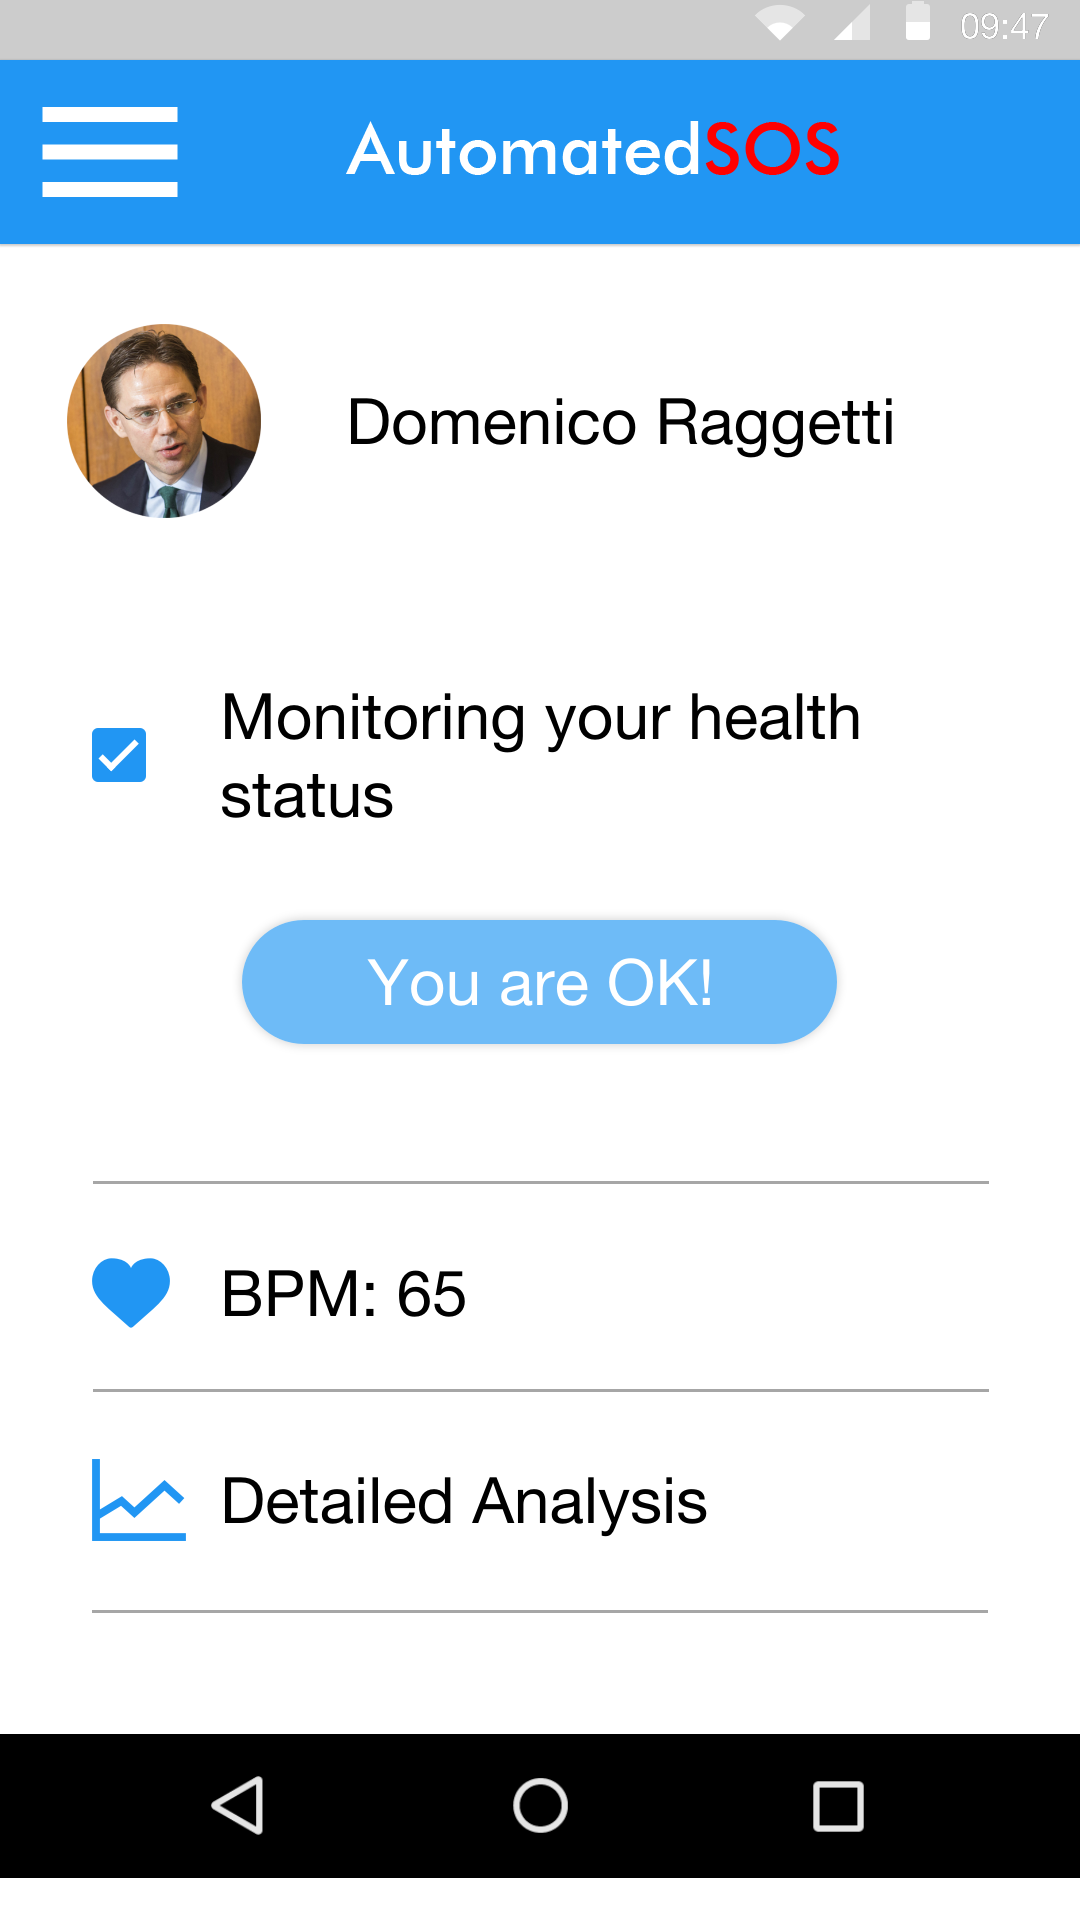
\includegraphics[width=160pt]{AutomatedSOS} 
    \caption{Regular health notification.}
    \label{fig:subim1}
    \end{subfigure}
    \begin{subfigure}{0.5\textwidth}
    \includegraphics[width=160pt]{AutomatedSOSemergency}
    \caption{Emergency notification.}
    \label{fig:subim2}
    \end{subfigure}
\caption{Smartphone interfaces of AutomatedSOS.}
\label{fig:image2}
\end{figure}

\vspace{1cm}

\begin{figure}[H]
    \centering
    \includegraphics[width=160pt]{AutomatedSOSSmartWatch}
    \caption{Smartwatch interface of AutomatedSOS.}
    \label{fig:my_label}
\end{figure}

\clearpage

\begin{figure}[H]
    \begin{subfigure}{0.5\textwidth}
    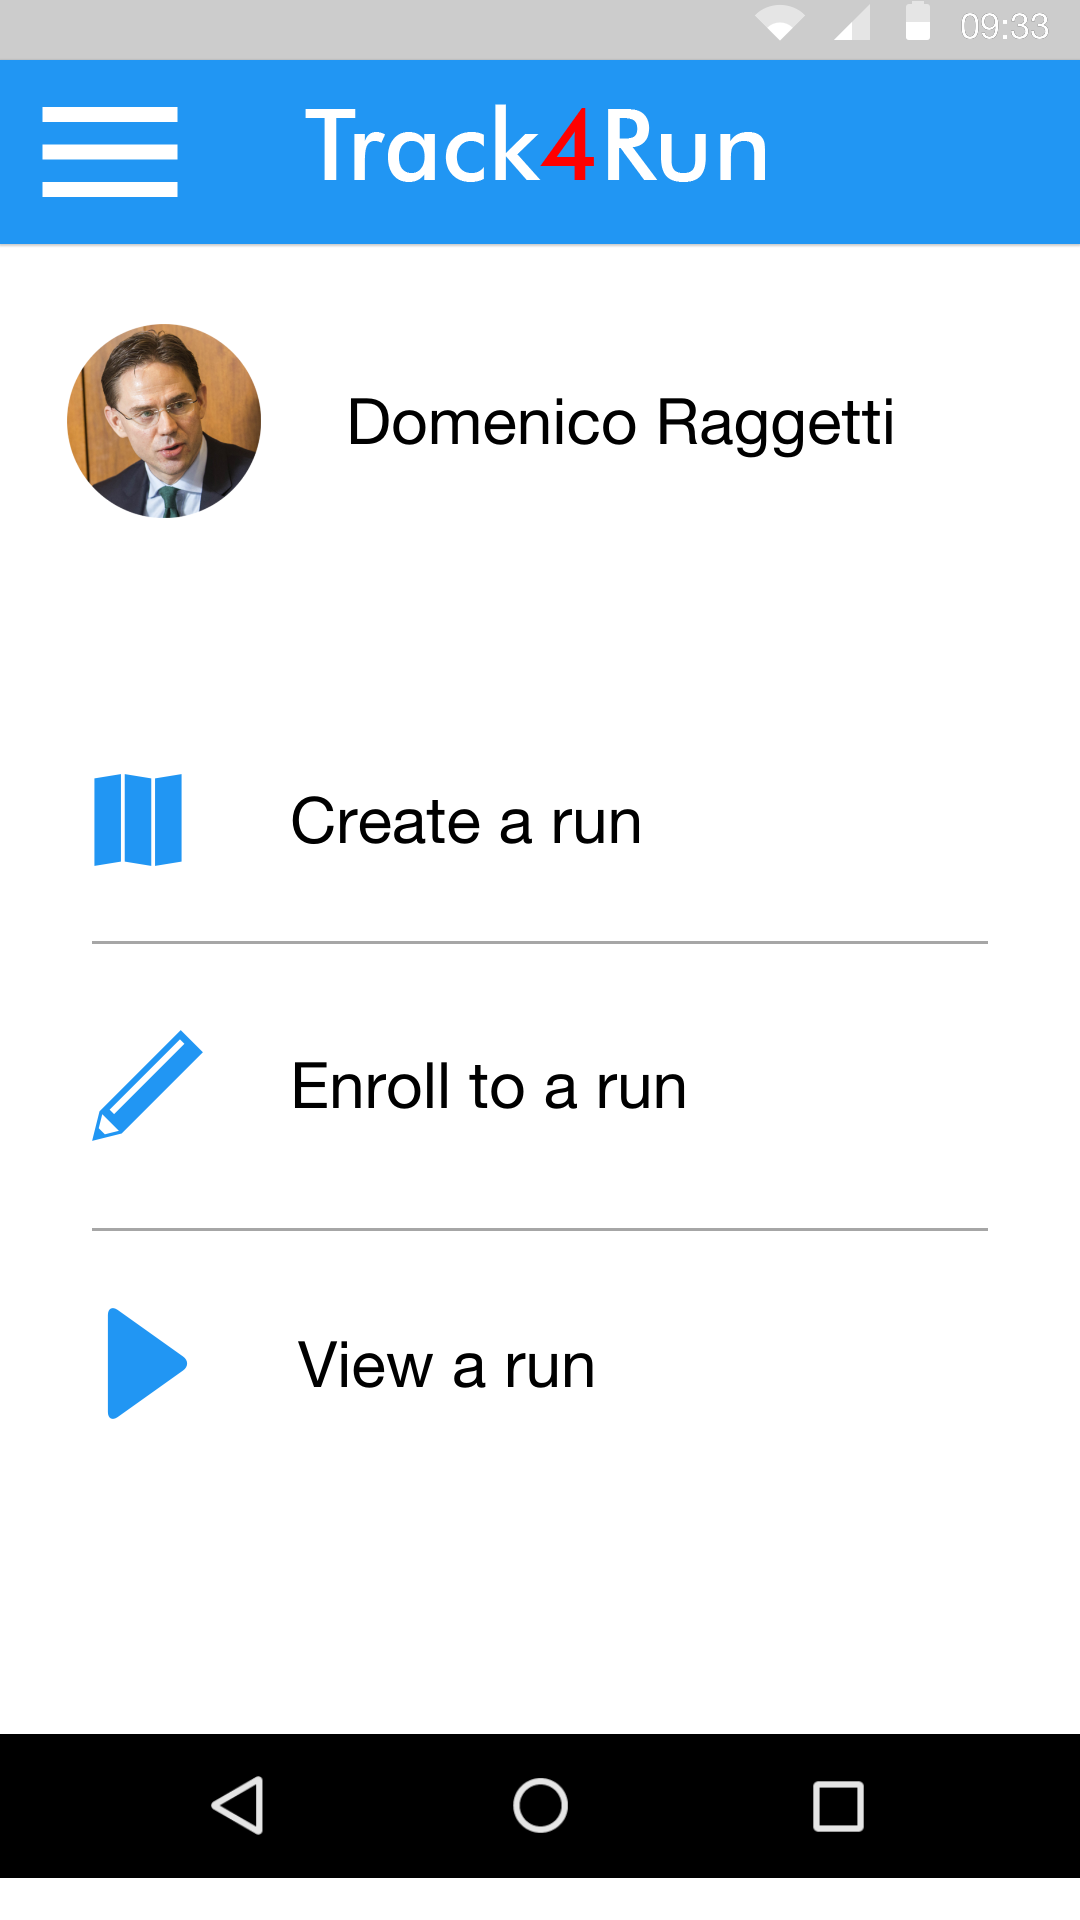
\includegraphics[width=160pt]{Track4RunHome} 
    \caption{Main page with all options.}
    \label{fig:subim1}
    \end{subfigure}
    \begin{subfigure}{0.5\textwidth}
    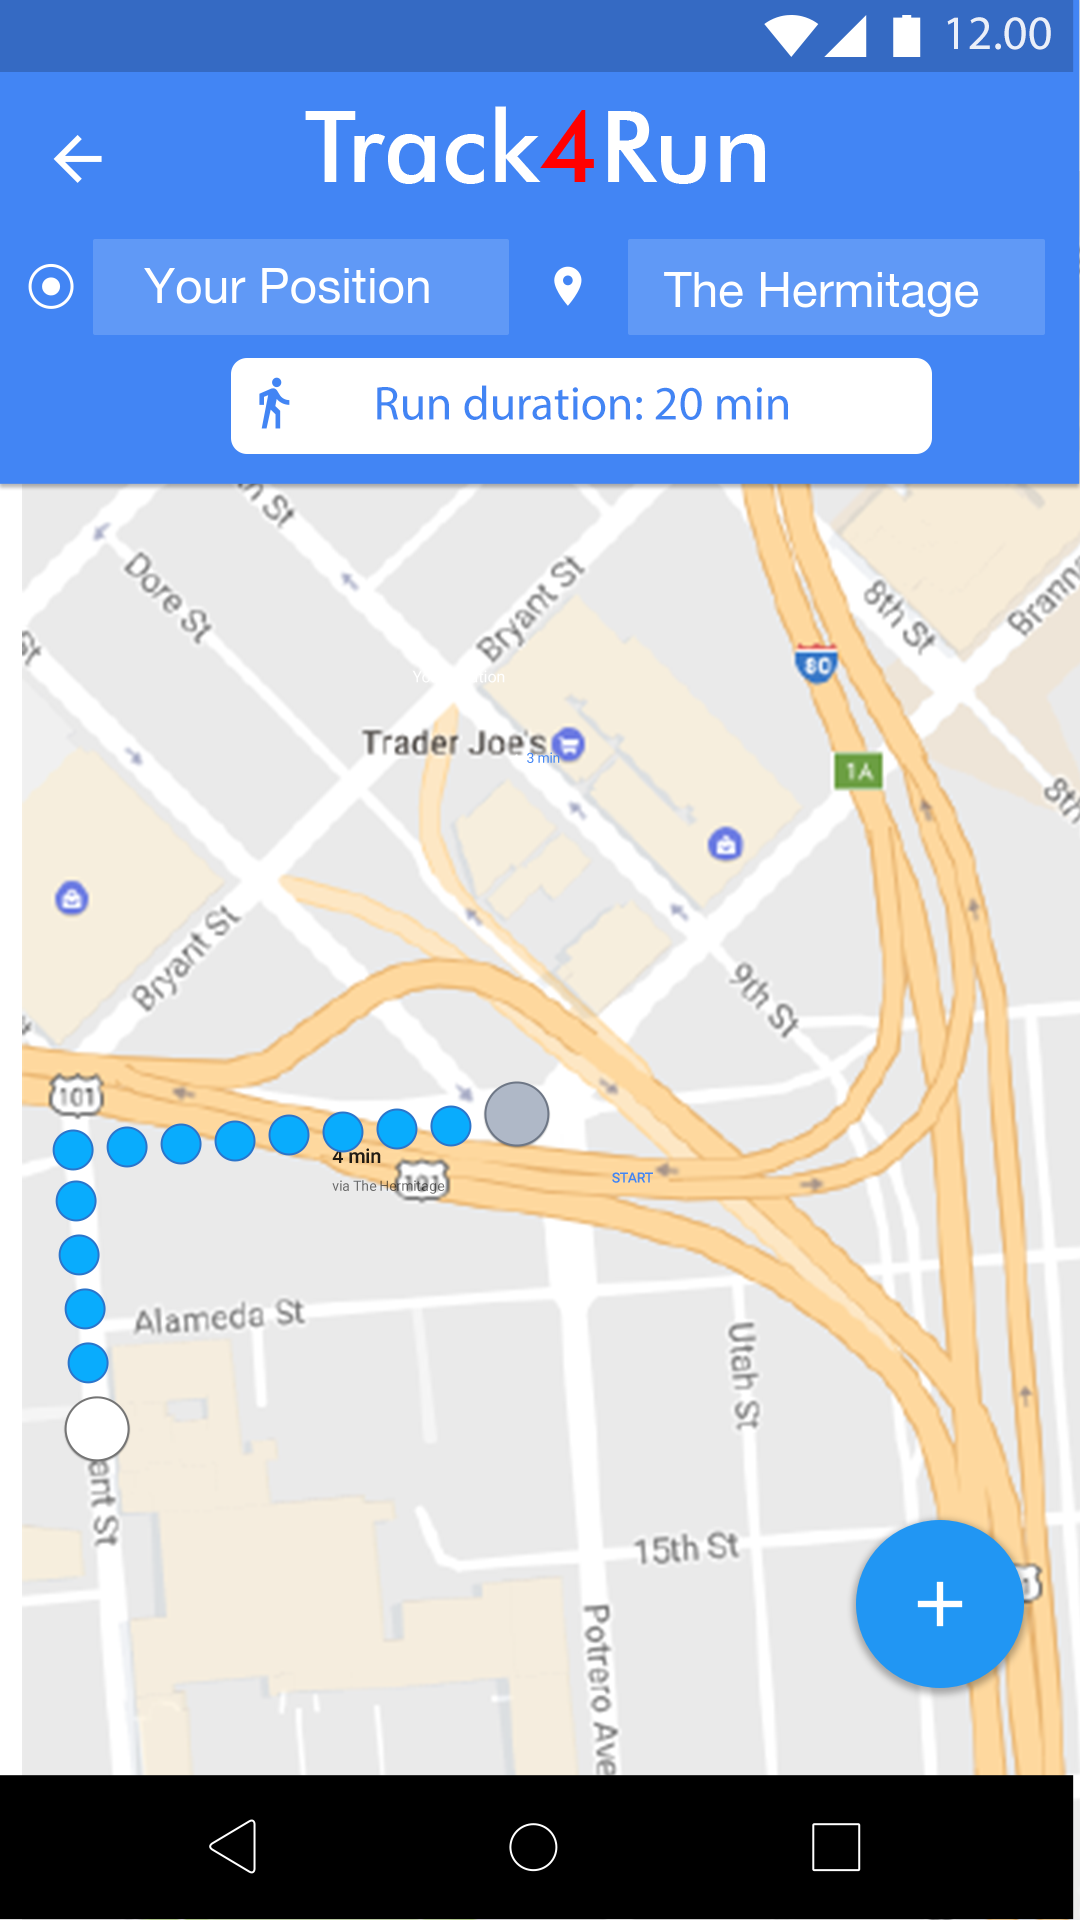
\includegraphics[width=160pt]{Track4Run}
    \caption{Selection of the path during the event creation.}
    \label{fig:subim2}
    \end{subfigure}
\caption{Smartphone interfaces of Track4Run.}
\label{fig:image2}
\end{figure}

\vspace{1cm}

\begin{figure}[H]
    \centering
    \includegraphics[width=160pt]{Track4RunSmartWatch}
    \caption{Smartwatch interface of Track4Run.}
    \label{fig:my_label}
\end{figure}

\clearpage

\subsubsection{Hardware Interfaces}

\paragraph{Data4Help:} The system should be a sever-based system made up of:
\begin{itemize}
    \item A main server (possibly distributed to guarantee better reliability and scalability) with a server OS to handle the main functions: permission and request managing, data managing, etc.
    \item A database to store the collected data (possibly in-source to preserve data sensibility).
    \item A DBMS to manage the database.
\end{itemize}
The Data4Help services are accessible from the users through a web browser or through mobile device applications of third parties.
The system, to collect data, exploits the devices of the users which use third parties services, these devices must integrate sensors in order to allow Data4Help to acquire data.

\paragraph{AutomatedSOS:} The system is based on a Client-Server architecture. It is composed by:
\begin{itemize}
    \item A server to provide the main functions: users' data managing and handle the emergency status and notify the ambulance dispatcher through the push notification external service.
    \item A mobile device with a supported OS (Android OS, iOS, Android Wear OS, etc.) where it is possible to install the AutomateSOS app. The device (Smartphone, smartwatch, smartwears, etc.) must respect the constraints that Data4Help requires.
\end{itemize}

\paragraph{Track4Run} Also this system is based on a Client-Server architecture. It is composed by:
\begin{itemize}
    \item A server to provide the main functions: runs managing, runners tracking, streaming for the spectators during the run.
    \item A mobile device with a supported OS (Android OS, iOS, Android Wear OS, etc.) where it is possible to install the Track4Run app. The device (Smartphone, smartwatch, smartwears, etc.) must respect the constraints that Data4Help requires.
\end{itemize}
\clearpage

\subsubsection{Software Interfaces}

\paragraph{Data4Help:} The interfaces needed from the system are:
\begin{itemize}
    \item A server OS to manage all the back-end functions. It has to implement REST API to communicate and transfer data with the mobile devices, the third parties' servers.
    \item A DBMS to manage the database.
\end{itemize}
Data4Help furthermore gives to the third parties a set of client-side APIs that provide an interface in order to connect their own client-side application with Data4Help services.

\paragraph{AutomatedSOS:} the system needs to manage the communication with Data4Help, to analyze the data and to communicate with the ambulance dispatcher and the communication between the app and the server. The software interfaces needed are:

\begin{itemize}
    \item Android OS, Android Wear OS or iOS for the client-side application.
    \item Data4Help API to access to services and receive data with Data4Help.
    \item REST API to communicate and transfer data on the web between the client app and the server.
    \item Interface with the Push Notification service to send reliable messages to the ambulance dispatcher.
\end{itemize}

\paragraph{Track4Run:} the system needs to manage the run events with the respective runners and spectators and let the spectators watch the run events on the map. Otherwise has to manage the communication with Data4Help and between the client app and the server. The interfaces needed are:

\begin{itemize}
    \item Android OS, android Wear OS or iOS for the client-side application.
    \item Data4Help API to access to the services and receive data with Data4Help.
    \item REST API to communicate and transfer data on the web between the app and the server.
    \item interface with the Google Maps API to manage the map for the runs.
\end{itemize}
\clearpage

\subsubsection{Communication Interfaces}

The system is based on a Client-Server architecture, in particular the communication between the different actors and elements of the system:
\begin{itemize}
    \item Data4Help Server and Data4Help API Client
    \item Third Parties/User and Data4Help
    \item AutomatedSOS Server and AutomatedSOS Client
    \item Track4Run Server and Track4Run Client.
\end{itemize}

The communication is based on: 
\begin{itemize}
    \item the REST API to make requests
    \item the AJAX API to transfer data.
\end{itemize}

The REST standard is recommended because is largely used on the web from the most of the devices and it guarantees better portability, maintainability and compatibility. \newline
Data4Help collects data from the users through its Client-side APIs which must be integrated in the third party software. Then the acquired data are provided to the Third Parties. Data4Help also takes on the responsibility of managing requests and permissions. \clearpage

This is a possible configuration of the system:
\begin{figure}[H]
    \centering
    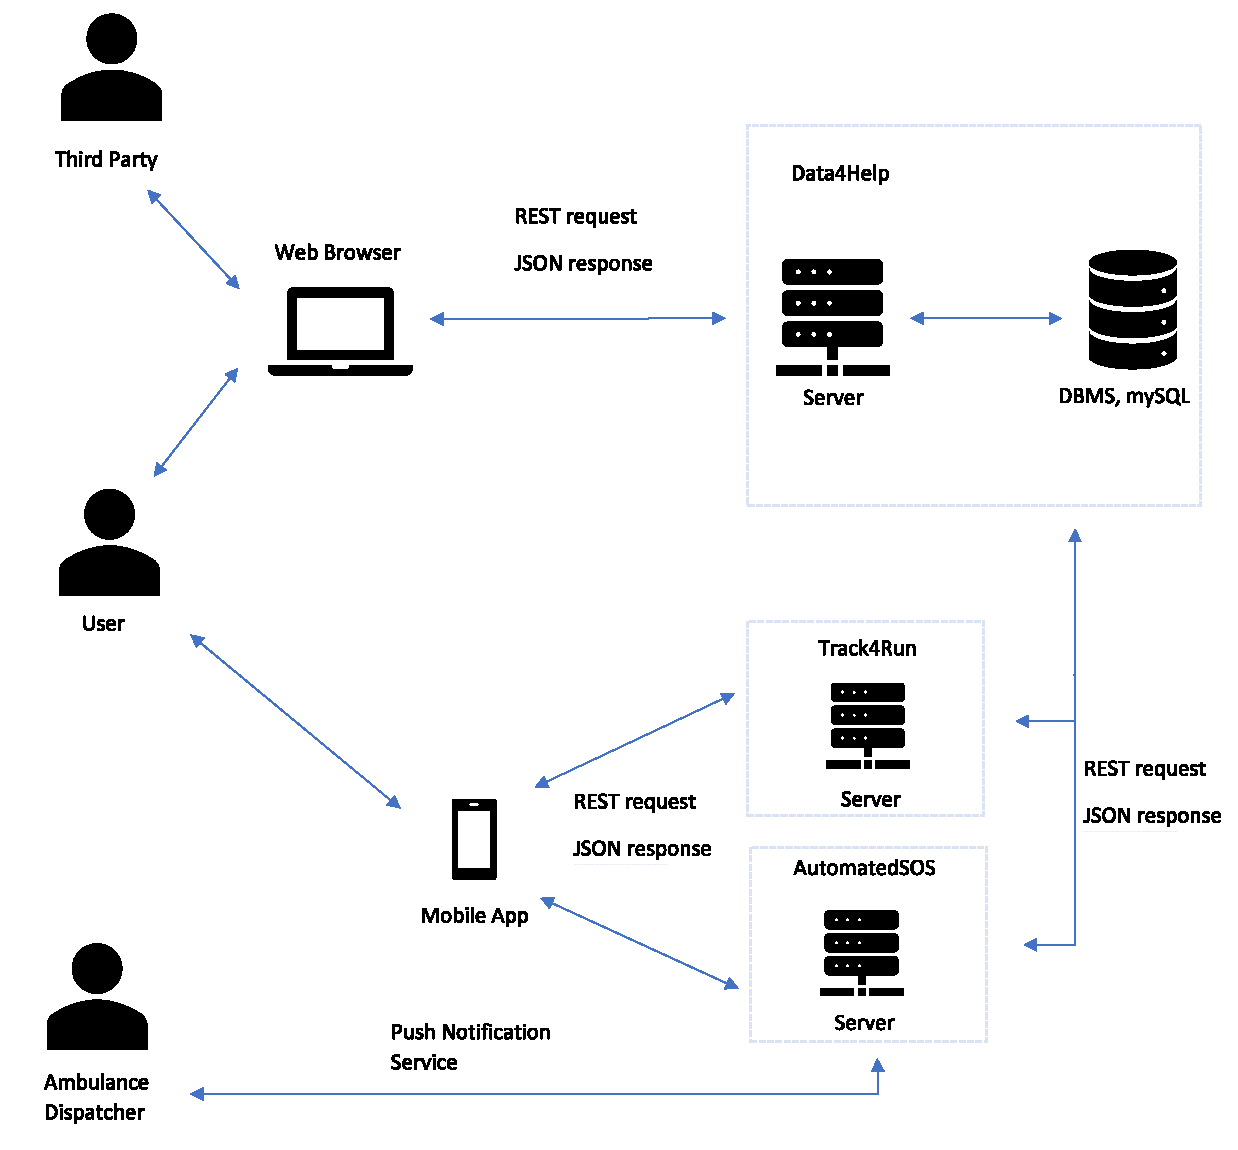
\includegraphics[width=\textwidth]{communicationInterfaces1}
    \caption{Communication schema of the whole system.}
    \label{fig:my_label}
\end{figure}

This is the schema of the communication by which data are collected and dispatched among third parties' app, Data4help API, third parties' server and Data4Help server services:

\begin{figure}[H]
    \centering
    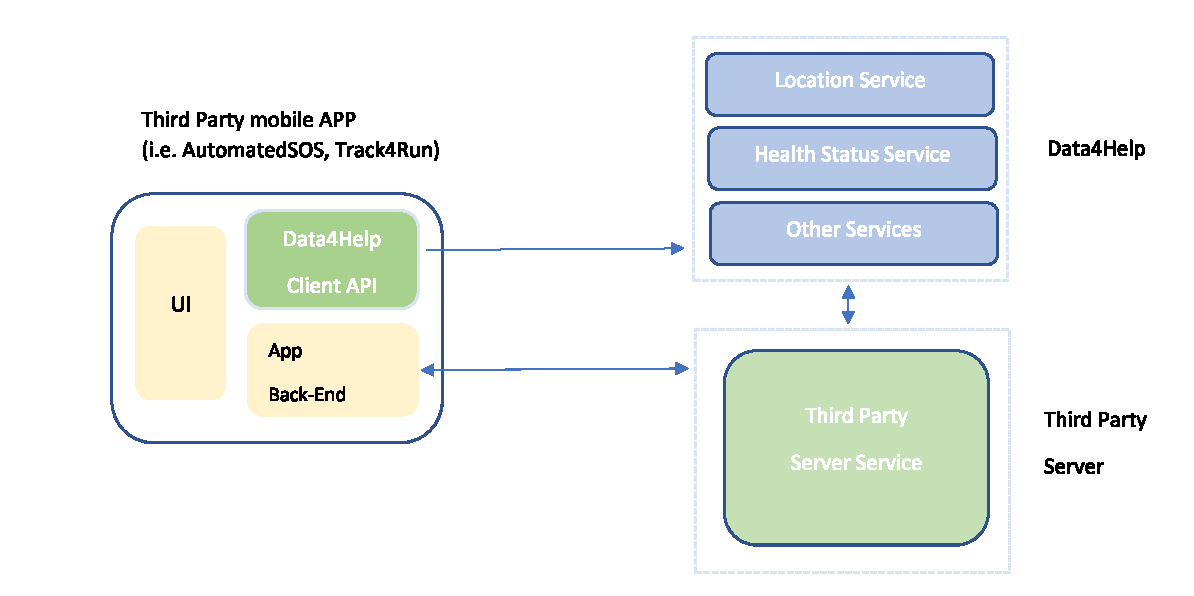
\includegraphics[height=150pt]{communicationInterfaces2}
    \caption{Data collection and trade of Data4Help.}
    \label{fig:my_label}
\end{figure}

\clearpage

\subsection{Scenarios}

%Data4Help
\subsubsection{Bran and the sign up}
Bran, a 17-years old guy, likes athletics and, in particular, running, which usually performs with his friend Rickon. \newline
During the last training, Rickon has shown to him Runnister, a new Android app, which explains some exercises for the warm up and monitors the users' health status to warn about possible damaging workouts. The app leans on a system which collects data, called Data4Help, and to which is necessary to be registered to. \newline
Bran, enthusiastic, runs home and turns on the laptop, with the purpose to register to Data4Help. Enters in the homepage of the site and clicks the "Sign Up" button. Then completes the fields with his personal information, providing an email and the password. He also checks the terms of conditions, giving the consensus to the treatment of personal anonymized data. Finally, he finishes the registration and comes back automatically to the homepage.

\subsubsection{Runnister's businnes plan}
The Runnister company, owner of the namesake application for mobile devices, wants to enlarge its range of users and start to cover a wider area. For this reason needs Data4Help service which can provide information about health status parameters of its users in the Dothraki District. \newline
First of all, the Runnister's agent accesses to the web site and logs in (Runnister has already used the service in the past and doesn't need to register anymore). He clicks on "Data Request" button and selects the one-time typology. Then selects the filter that must be applied to obtain data coming from a certain region (in this case "Dothraki District"). After that, he waits the confirmation to the request from Data4Help. \newline
Unfortunately, users of Data4Help residing in "Dothraki District" aren't enough to satisfy the threshold which preserves the anonymity. The request is refused and Runnister's agent receives the notification of the refusal.

\subsubsection{Breakfast with Starkbucks}
Starkbucks is a company that makes statistics on the variations of health parameters generated from a non-healthy nutrition. For the next winter it has planned a analysis on the effects of the coffee on adult people's heartbeat and, to conduct this research, it needs to periodically acquire relevant data. Hence, it decides to ask Data4Help to get them. \newline 
After the company registration on the web site, the operator of Starkbucks, logged in the personal area, clicks on "Data Request" button and selects the acquirement of data through the subscription way. Then he chooses to pick users' data which have been collected only in the time slot between 7:00 and 9:00, i.e. the breakfast period. Then he waits for the confirmation. After some hour the operator receives the notification of confirmation and Starkbucks starts to periodically obtain the required data. \newline
In March, at the end of the winter, Starkbucks has already collected enough data, so decides to unsubscribe from the service and stops to receive updates from Data4Help. 

\subsubsection{The worries of Brienne}
Hospitarly is an institute which conducts researches on diseases and cancer, offering to its patients the possibility to remain always updated on their own health condition. To integrate user's information, the company takes more precise data from Data4Help, but it must have the consensus of the user. \newline
Brienne is a middle-aged woman which has passed some sad moments for her health problems. For this reason, she wants to keep herself monitored and decides to use Hospitarly service. At the moment, she has already registered to Data4Help. \newline
During the sign up to the service, she receives the proposal to allow Data4Help to share her personal data with Hospitarly, in order to permit a richer and more updated analysis. She accepts the request. \newline
From this point, Hospitarly can ask whenever it needs information to Data4Help about Brienne's status and provide a more accurate service to its user.

%automatedSOS
\subsubsection{The walk of uncle Jamie}
Uncle Jamie has recently gone through a bad period, caused by his heart illness. To prevent another relapse, the doctor has advised him to get some walk everyday and install in his smartwatch an application, called AutomatedSOS, that provides an immediate rescue if his health parameters decrease under a given threshold. He listen to his doctor' advise and downloads the application. \newline
After the registration to AutomatedSOS and the previous sign up to Data4Help, uncle Jamie decides to try the new software during a walk. He wears his smartwatch and look at the AutomatedSOS interface, which reports a regular health status, with a normal heartbeat. Pleased with that, he starts his walk. \newline
Suddenly, in the middle of the walk, the smartwatch starts to   flash and emit an alert noise. Uncle Jamie watches his clock and understands that he is having some health issue. Immedialtely, he begins to have blurry vision and he collapses on the ground. \newline
The last sound he hears is a notification from his smartwatch that an ambulance has been sent to rescue him.

%track4run
\subsubsection{Forrest, the run planner}
Forrest is a young man which loves running. He recently learns about a new application, called Track4Run, with the purpose to allow its users to organize run event. Excited for the new discovery, he invites a lot of friend to download the application and tries to set a run event for the next week. \newline
After the registration to Track4Run and the previous sign up to Data4Help, he launches the app. First of all, he clicks on "Create a run" button, choosing starting and ending point and the path in the middle from the map. Then, he gives the day and the hour at which the run will start. Finally, he receives the notification of the event creation and the opening of the subscription period. \newline
Now Forrest has only to enroll in his run event as a runner and wait until the day of the run. 

\subsubsection{Jon and his training}
Jon is an autonomous athlete that has never joined in a sport association. To test himself he uses to access to Track4Run to find out some run events in which freely enroll. Now he wants to look for an event for the next week in South Carolina. \newline
First of all, he launches Track4Run application from his phone and selects the "Enroll in a run" button. Then Jon selects the city, in this case Beaufort, and chooses the run event that fits better with his appointments. He finds the Forrest's run and decides to enroll himself in that run. \newline
Jon is eventually registered as a runner in the event database and he will receive a notification just before the beginning of the event.

\subsubsection{A runner as brother}
To be updated on the placement of his brother Jon, Arya, which has already downloaded Track4Run on is device, decides to watch the run during is progression. \newline
First of all, at the beginning of the run Arya launches Track4Run from her smartphone and selects the "View a run" button. Therefore, she indicates the city in which the run is held and chooses the desired run from the list of that is appeared. After that, on her phone appears the interface of the real-time map with the position of the runners, between which there is also Jon. \newline
Arya watches the event until the end, being witness of his brother defeat.

\clearpage

\subsection{Functional Requirements}

\subsubsection{Specific Requirements}
\begin{enumerate}[label*=\bf{G.\arabic*}]
    
    %Data4Help
    \item \textbf{Allow customers’ registration.}
    \begin{enumerate}
        \item [D.2] The personal information given by the user (age, address, gender, etc.) and the third parties (name, address, etc.) are correct and the account is not used by other people. 
    \end{enumerate}
    
    \begin{enumerate}[label*=\bf{.\arabic*}]
        \item \textbf{Registration can be done as individual user.}
        \begin{enumerate}
            \item [R.1] People can create a user account selecting username, password, giving personal information (age, address,gender) and allow to share their anonymized data.
            
        \end{enumerate}
        
        \item \textbf{Registration can be done as third party.}
        \begin{enumerate}
            \item [R.2] It is possible to create a third party account selecting username and password and giving the company main information.
        \end{enumerate}
    \end{enumerate}
    
    \item \textbf{Third parties can receive anonymized data.}
            
    \begin{enumerate}
        \item [R.3] Data4Help allows third parties to request anonymized data acquired from a filtered group of users (by age, gender, address, etc.).
        \item [R.4] Data4Help collects data from registered users and gives access to third parties only if the number of individuals whose data satisfy the request is higher than 1000.
        \item [D.2] The personal information given by the user (age, address, gender...) and the third parties are correct and the account is not used by other people.
    \end{enumerate}
        
        
    \item \textbf{Third parties can subscribe to the service in order to periodically receive new data.}
    
    \begin{enumerate}
        \item [R.5] Data4Help allows third parties to join the subscription service for an indeterminate period and then, in case, unsubscribe from that.
        \item [R.6] Data4Help provides new data, checking each time if groups data satisfy the given constraint (number of individuals not lower than a thousand).
        \item [R.7] Data4Help keeps track of the associations between third parties subscriptions and the required group data.
    \end{enumerate}
    
    
    \item \textbf{Third parties can receive specific person's data.}
            
    \begin{enumerate}
        \item[R.8] Data4Help allows third parties to require specific person's data. 
        \item [R.9] Data4Help forwards requests from third parties to the demanded users which can accept or refuse to share their own personal data.
        \item [R.10] Data4Help keeps track of the connections between a specific user and the third parties which can access to his/her data.
        \item [R.11] Data4Help allows third parties to have access to demanded users' data each time they need them.
    \end{enumerate}
            
        
    %AutomatedSOS
    \item \textbf{Users' health status is continuously checked in AutomatedSOS and if it is below a certain threshold values an ambulance is called within 5 seconds and sent to the user's position.}

    \begin{enumerate}
        \item [D.1] The data collected from the devices (position and health status) are reliable, accurate and in real time.
        \item [R.12] Users' health and position information received by Data4Help are analyzed and compared with the threshold values.
        \item [R.13] In case of emergency (the health status values overcome the threshold) a request for an ambulance is sent to the ambulance dispatcher in 5 seconds, containing the user's information.
        \item [D.3] Ambulance call and information about patients' status and position are correctly dispatched to the ambulance contact center.
    \end{enumerate}
    
    %Track4Run
    \item \textbf{Users can organize a run.}
    
    \begin{enumerate}
        \item [R.14] Users select the day, the hour at which the run begins, the starting point, the ending point and the path for the run.
        \item [R.15] The run event is stored in the system in order to be managed during its lifecycle.
        \item [D.4] Information and data (places, maps, paths, etc.) received from external services are correct and reliable.
    \end{enumerate}
    
    \item \textbf{Users can organize a run.}
    
    \begin{enumerate}
        \item [R.16] Users can browse among the available runs and see their information.
        \item [R.17] Users can choose a run and register to it as a runners.
% NON-FUNCTIONAL         \item [R.12] Users can choose to see the available runs filtering them by city and/or date. 
        \item [R.18] The system saves the enrolled users as runners and keeps track of the association with the run event.
    \end{enumerate}
    
    \item \textbf{Users can be spectators of a run seeing the participants' position on a map.}
    
    \begin{enumerate}
        \item [R.14] The system keeps track of all the enrolled runners' position during the run.
        \item [R.15] Users who require to watch a run are saved as spectators to the run event.
        \item [R.16] Track4Run offers the possibility to see the run live through a map.
        \item [D.4] Information and data (places, maps, paths, etc.) received from external services are correct and reliable.
    \end{enumerate}
    
\end{enumerate}
\clearpage



\paragraph{Use cases}

\subsubsection{User's sign up}

\begin{center}
\begin{tabular}{|l || p{8cm} ||}
    \hline\bf{ACTORS} & User \\ 
    \hline
    \bf{ENTRY CONDITIONS} & No entry condition needed  \\ 
    \hline
    \bf{EVENTS FLOW} & \begin{itemize}[noitemsep, topsep=0cm, leftmargin=*] \vspace{-0.2cm}
        \item[1.] User opens Data4Help web page and press “Sign Up” button.
        \item[2.] User inserts personal information (name, address, age, gender, fiscal code).
        \item[3.] User selects email and password.
        \item[4.] User allows terms of conditions to share anonymized data with Data4Help.
        \item[5.] User completes the registration.
        \item[6.] The system saves the new account.
    \end{itemize}\\ 
    \hline
    \bf{EXIT CONDITIONS} & The user is successfully registered and his/her data can be collected by Data4Help. He/she is redirected to the homepage. \\ \hline
    \bf{EXCEPTIONS} & \begin{itemize}[noitemsep, topsep=0cm, leftmargin=*] \vspace{-0.2cm}
        \item[1.] The user doesn’t fill all the mandatory fields with valid data.
        \item[2.]The inserted email is already used by another user.
        \item[3.] The user doesn’t allow the term of condition and he/she can’t complete the registration.
    \end{itemize}
    \\ \hline \hline
\end{tabular}
\end{center}

\vspace{0.5cm}

\subsubsection{One-time request for anonymous data}
\begin{center}
\begin{tabular}{|l || p{8cm} ||}
    \hline\bf{ACTORS} & Third Party \\ \hline
    \bf{ENTRY CONDITIONS} & This use case starts when the third party is registered, successfully logged in to Data4Help and is connected to the web page.\\ \hline
    \bf{EVENTS FLOW} & \begin{itemize}[noitemsep, topsep=0cm, leftmargin=*] \vspace{-0.2cm}
        \item[1.] The Third Party click on "Data Request" button.
        \item[2.] The Third Party selects to require anonymous data with a one-time request.
        \item[3.] The Third Party selects the filter that must be applied to gather users.
        \item[4.] The system checks if the request can be accepted to guarantee the users' anonymity or not.
        \item[5.] Third party receives the confirmation to the request.
    \end{itemize}
    \\ \hline
    \bf{EXIT CONDITIONS} & The request is accepted and anonymized data are sent to the Third Party.\\ \hline
    \bf{EXCEPTIONS} & The number of users satisfying the filter is smaller than 1000, then the request is refused. 
    \\ \hline \hline
\end{tabular}
\end{center}

\subsubsection{Subscription to anonymous data set}
\begin{center}
\begin{tabular}{|l || p{8cm} ||}
    \hline\bf{ACTORS} & Third Party \\ \hline
    \bf{ENTRY CONDITIONS} & This use case starts when the third party is registered, successfully logged in to Data4Help and connected to the web page.\\ \hline
    \bf{EVENTS FLOW} & \begin{itemize}[noitemsep, topsep=0cm, leftmargin=*] \vspace{-0.2cm}
        \item[1.] The Third Party clicks on "Data Request" button.
        \item[2.] The Third Party selects to require anonymous data with a subscription request.
        \item[3.] The Third Party selects the filter that must be applied to gather users.
        \item[4.] The system checks if the request can be accepted to guarantee the users' anonymity or not.
        \item[5.] The Third Party receives the confirmation to the request.
        \item[6.] The Third Party is periodically notified with new anonymous data about the selected users' group. 
    \end{itemize}
    \\ \hline
    \bf{EXIT CONDITIONS} & The Third Party decides to unsubscribe from the service and stops to receives periodical updates.\\ \hline
    \bf{EXCEPTIONS} &\begin{itemize}[noitemsep, topsep=0cm, leftmargin=*] \vspace{-0.2cm}
        \item[1.] The number of users satisfying the filter is smaller than 1000, then the request is refused.
        \item[2.] During the service supply the number of users in the group decreases under 1000 entities, so the service is stopped.
    \end{itemize}
    \\ \hline \hline
\end{tabular}
\end{center}

\vspace{0.5cm}

\subsubsection{Request for specific user's data}
\begin{center}
\begin{tabular}{|l || p{8cm} ||}
    \hline \bf{ACTORS} & Third Party, User \\ \hline
    \bf{ENTRY CONDITIONS} & This use case starts when the Third Party is registered, successfully logged in to Data4Help and connected to the web page.   \\ \hline
    \bf{EVENTS FLOW} & \begin{itemize}[noitemsep, topsep=0cm, leftmargin=*] \vspace{-0.2cm}
        \item[1.] The Third Party clicks on "Data Request" button.
        \item[2.] The Third Party selects the option "Require Individual Data".
        \item[3.] The system sends a request to the users whose the Third Party needs data.
        \item[4.] Once the user has allowed to acquire his/her personal data, a confirmation to the request is sent to the Third Party.
    \end{itemize}
    \\ \hline
    \bf{EXIT CONDITIONS} & The Third Party can require and access to user's personal data. \\ \hline
    \bf{EXCEPTIONS} & The user doesn't allow to share personal data and the system rejects the request of the Third Party.
    \\ \hline \hline
\end{tabular}
\end{center}

%AutomatedSOS
\subsubsection{Alert emergency status}
\begin{center}
\begin{tabular}{|l || p{8cm} ||}
    \hline \bf{ACTORS} & User, Ambulance Dispatcher \\ \hline
    \bf{ENTRY CONDITIONS} & This use case starts when the user is registered and logged in to AutomatedSOS on his/her device, moreover has allowed the permission to share personal data with this third party. \\ \hline
    \bf{EVENTS FLOW} & \begin{itemize}[noitemsep, topsep=0cm, leftmargin=*] \vspace{-0.2cm}
        \item[1.] The system receives the user's health data collected from his/her device by Data4Help.
        \item[2.] The system analyzes the data and notices that the health status is under the safety threshold.
        \item[3.] The system notifies the emergency to the Ambulance Dispatcher within 5 seconds, reporting the user's health status and position.
        \item[4.] The system sends a warning to the user's device to notify that the health status is under the threshold and that an ambulance has been called to reach his/her position.
        \item[5.] The system receives the acknowledgement from the Ambulance Dispatcher which notifies that an ambulance has been sent.
        \item[6.] The system notices that the health status has became regular again.
    \end{itemize}
    \\ \hline
    \bf{EXIT CONDITIONS} & The system keeps monitoring the user's health status and position. \\ \hline
    \bf{EXCEPTIONS} & The Ambulance Dispatcher doesn't send any confirmation and the system continues to periodically notify it with the alert status until a confirmation is received.
    \\ \hline \hline
\end{tabular}
\end{center}

\clearpage

%Track4Run
\subsubsection{Creation of a run event}
\begin{center}
\begin{tabular}{|l || p{8cm} ||}
    \hline\bf{ACTORS} & User \\ \hline
    \bf{ENTRY CONDITIONS} & This use case starts when the user is registered and logged in to Track4Run on his/her device, moreover has allowed the permission to share personal data with this third party.  \\ \hline
    \bf{EVENTS FLOW} & \begin{itemize}[noitemsep, topsep=0cm, leftmargin=*] \vspace{-0.2cm}
        \item[1.] The user selects the "Create a run" button.
        \item[2.] The user chooses the starting point, the ending point and the path on the map.
        \item[3.] The user selects the day and the starting time of the run event.
        \item[4.] The system confirms the run event creation to the user and saves it in the database.
    \end{itemize}
    \\ \hline
    \bf{EXIT CONDITIONS} & The run event is created and the track4Run users can enroll to the event.\\ \hline
    \bf{EXCEPTIONS} &  The selected path or the starting/ending point is unavailable for a run. The system lets the user choose an available one. \\ \hline \hline
\end{tabular}
\end{center}

\vspace{0.5cm}

\subsubsection{Enrollment in a run}
\begin{center}
\begin{tabular}{|l || p{8cm} ||}
    \hline\bf{ACTORS} & User \\ \hline
    \bf{ENTRY CONDITIONS} & This use case starts when the user is registered and logged in to Track4Run on his/her device. Moreover has allowed the permission to share personal data with this third party and at least a run event has been already created. \\ \hline
    \bf{EVENTS FLOW} & \begin{itemize}[noitemsep, topsep=0cm, leftmargin=*] \vspace{-0.2cm}
        \item[1.] The user selects the "Enroll in a run" button.
        \item[2.] The user selects the city that interests him/her.
        \item[3.] The system shows the list of available runs in the selected city.
        \item[4.] The user selects the run event he/she wants to enroll.
        \item[5.] The system saves the user in the run event as a runner.
        \item[6.] The system notifies the user when the run is going to start.
    \end{itemize}
    \\ \hline
    \bf{EXIT CONDITIONS} & The user is correctly enrolled to the run event and can take part to it. \\ \hline
    \bf{EXCEPTIONS} & There are no available runs. 
    \\ \hline \hline
\end{tabular}
\end{center}

\subsubsection{Watch a run}
\begin{center}
\begin{tabular}{|l || p{8cm} ||}
    \hline\bf{ACTORS} & User \\ \hline
    \bf{ENTRY CONDITIONS} & This use case starts when the user is registered and logged in to Track4Run on his/her device, on the main page. Moreover has allowed the permission to share personal data with this third party and at least a run event has been already created. \\ \hline
    \bf{EVENTS FLOW} & \begin{itemize}[noitemsep, topsep=0cm, leftmargin=*] \vspace{-0.2cm}
        \item[1.] The user selects the "View a run" button.
        \item[2.] The user selects the city that interests him/her. 
        \item[3.] The system shows the list of available runs in the selected city.
        \item[4.] The user selects the run event he/she wants to watch.
        \item[5.] The system saves the user in the run event as a spectator.
    \end{itemize}
    \\ \hline
    \bf{EXIT CONDITIONS} & The user can watch on his/her device the map with the path and the runners positions updated in real time. \\ \hline
    \bf{EXCEPTIONS} & \\ \hline \hline
\end{tabular}
\end{center}

\clearpage

\subsection{Performance Requirements}

\paragraph{Data4Help} The system is designed to provide a large number of users and third parties moreover it is necessary to guarantee that the data is acquired, analyzed and made available to third parties in reasonable times. Especially individual data has to be provided to the third parties as soon they require them (periodically or even with real time updates).

\paragraph{AutomatedSOS} This is a non-intrusive SOS service that needs to monitor the user health status in every moment. Once user's data are received from Data4Help the system must analyze the values and compare them with safe thresholds in a short time. If the values are under the fixed thresholds the system must warn the ambulance contact center in 5 seconds to send an ambulance to the user location.

\paragraph{Track4Run} the system must be able to manage a large number of users enrolled in a single run event (the number of runners for a single run can be between less then 10 and almost 1000), a large number of run events for several cities and it must guarantee that the spectators can watch the runners' position on the map with a real time update.
\clearpage

\subsection{Design Constraints}

\subsubsection{Standards Compliance}

Individual people to get access to Data4Help, AutomatedSOS and Track4Run services must sign in to Data4Help. By registering to Data4Help the user must allow the permissions to share anonymazed data with Data4Help and third parties, unless he/she can't complete the registration.
AutomatedSOS and Track4Run are third parties actors developed by TrackMe and, as such, they have to require to Data4Help the permission to receive individual data from the users.
If an user wants to use AutomatedSOS and Track4Run services must accept the permissions to share individual data with them, unless their data can't be dispatched from Data4Help to the specific third party and the third party service can't be provided.

\subsubsection{Hardware Limitations}
\textbf{Data4Help} doesn't require specific hardware limitations for third parties. Users should use mobile devices with sensors useful for collecting data (GPS, cardiac pulse sensor, accelerometer, camera, light sensor) even if they are not strictly required. The only necessary requirement is that the device must have an internet connection (possibly fast):
\begin{itemize}
    \item 3G/4G internet connection
\end{itemize}

\noindent The hardware requirements for \textbf{AutomatedSOS} users' device, to collect the health information are:
\begin{itemize}
    \item 3G/4G internet connection
    \item GPS
    \item Cardiac pulse sensor, other health sensors
\end{itemize}
\noindent The hardware requirements for \textbf{Track4Run} users' devices are:
\begin{itemize}
    \item 3G/4G internet connection
    \item GPS
    \item Device that supports Google maps API
\end{itemize}

\clearpage

%Design constraints end

\subsection{Software System Attributes}

\subsubsection{Reliability} 

\paragraph{Data4Help} The system must be able to collect data from the users and guarantee the services to the third parties.
Third parties can request users' data with arbitrary frequency, also in "real-time". The system to guarantee a good and trusty service should not have failure and long period of time in which the functions are not provided to customers, specially for individual data requests. Infrequent short periods of time of unavailability may be tolerated (at most a few ongoing minutes).

\paragraph{AutomatedSOS} The service must acquire users' data from Data4Help and monitor the health status in real time (24h) to guarantee the health care in case of emergency. The system should not have failure that lasts for long period of time (it can be tolerated at most for a few minutes) and the status analysis, once the data are received from Data4Help, must be performed and completed in very short time to guarantee the time consistency of the health status.

\paragraph{Track4Run} The service must be guaranteed to the users during the entire day, letting them to manage and enroll to runs. In particular, in order to guarantee a good quality of service, during the runs it is needed an high level of location accuracy. The system should not have long period of unavailability especially in the day time and in the evening, the periods with the higher number of customers connected.

\vspace{0.5cm}

\subsubsection{Availability}

\paragraph{Data4Help} The system must have an high availability to guarantee all the functions. Using the "hour-per-week"  (a week is composed by 168 hours) the system should have an availability greater or equal than 165/168 or using the "nines" metric the system should have an availability greater than 1 nine (> 0.9).

\paragraph{AutomatedSOS} Also the AutomatedSOS system must have an high level of availability, to provide a better service is preferable an availability of two nines (0.99) in the "nines" metric.

\paragraph{Track4run} The system should offer their service for the runners with an availability at least of 150/168, with the priority of availabilty for the the day time and evening hours.
\clearpage

\subsubsection{Security}

In all the software offered by TrackMe it is necessary to guarantee an high level of security, in order to respect the sensibility of the users' data.
All the communications must be encrypted and the information should be sent on secure channels.
Furthermore the data stored in the Data4Help database must be accessible only from entities which have the necessary permissions. 
Users and third parties can access to the services providing their credentials (username, password). 

\vspace{0.5cm}

\subsubsection{Maintainability}

A good level of maintainability, since it is approximately 75\% of the cost related to a project, should be guaranteed for the development of the system, so it has to be corrective, adaptive, perfective, and preventative and
must be avoided poor code quality, source code defects, excessive technical complexity and poorly documented code.

\vspace{0.5cm}

\subsubsection{Portability}

The system should have an high level of portability in order that TrackMe can guarantee its services to a wide range of devices and users.
Providing a set of API instead of creating a dedicated app for Data4Help is useful to achieve this goal, in fact the third parties can choose different OS and devices for developing their own services and application, integrating the Data4Help service with them.
\clearpage

\section{Formal Analysis Using Alloy}
    
    \section{Effort Spent}
    
    Davide Salaorni
    
    \begin{center}
    \begin{tabular}{|l | l |}
        \hline \bf{Purpose, Scope, Definitions} & 1 \\ \hline
        \bf{Product Perspective and Functions, Assumptions,Scenarios}  & 4 \\ \hline
        \bf{External Interfaces} & 3 \\ \hline
        \bf{Functional Requirements} & 11 \\ \hline
        \bf{Design Constraint} & 3\\ \hline
        \bf{Software System Attributes} & 1 \\ \hline
        \bf{Alloy} & 9 \\ \hline
    \end{tabular}
\end{center}

\noindent  Luca Terracciano
    
        \begin{center}
    \begin{tabular}{|l | l |}
        \hline \bf{Purpose, Scope, Definitions} & 2 \\ \hline
        \bf{Product Perspective and Functions, Assumptions,Scenarios}  & 3 \\ \hline
        \bf{External Interfaces} & 4 \\ \hline
        \bf{Functional Requirements} & 9 \\ \hline
        \bf{Design Constraint} & 2\\ \hline
        \bf{Software System Attributes} & 3 \\ \hline
        \bf{Alloy} & 9 \\ \hline
    \end{tabular}
\end{center}

    \noindent Manuel Trivilino
    
        \begin{center}
    \begin{tabular}{|l | l |}
        \hline \bf{Purpose, Scope, Definitions} & 1 \\ \hline
        \bf{Product Perspective and Functions, Assumptions,Scenarios}  & 2 \\ \hline
        \bf{External Interfaces} & 5 \\ \hline
        \bf{Functional Requirements} & 9 \\ \hline
        \bf{Design Constraint} & 3 \\ \hline
        \bf{Software System Attributes} & 3 \\ \hline
        \bf{Alloy} & 9 \\ \hline
    \end{tabular}
\end{center}
    
    
    \section{References}

    \subsubsection{Used Tool}

    \begin{itemize}
        \item MagicDraw (diagrams)
        \item Alloy Analyzer 5.0
        \item Overleaf LaTex Editor
        \item gitHub
        \item Proto.io (mockups)
        \item Adobe Photoshop
        \item Visual Studio Code
        
    \end{itemize}
    
    \begin{itemize}
        \item Mandatory Project Assignment AY 2018-2019
        \item ISO/IEC/IEEE 29148 dated Dec 2011
        \item Alloy Documentation http://alloytools.org/documentation.html
        \item Slides: Alloy, Use of Alloy in RE
        \item LaTex Documentation: https://www.latex-project.org/help/documentation/
        
    \end{itemize}

    
    \end{document}
